\documentclass[11pt]{article}
\usepackage[margin=0.78in]{geometry}
\usepackage{amsmath,amssymb,graphicx,booktabs,hyperref}
\setlength{\parindent}{0pt}\setlength{\parskip}{6pt}
\begin{document}
{\LARGE Bounded twist relations and retained witnesses}\\
2026-10-30 \quad PR2381 \quad exact finite native study

\textbf{Actual source and twist.} Over $\mathbf F_{13}$,
$E:y^2=x^3+x+4$, $T:y^2=x^3+4x+6$, the $d=2$ monic twist.
$P=(0,2)$ maps to $U=(8,11)$, both order7, using the prior checked
coordinate map $\Phi$ and inverse $I=[4]D$ on seven-torsion.
No generic rational-point twist isomorphism or target-log lookup is assumed.

\textbf{Full fixed scope in each instrument.} All16 canonical/matched/pullback
factor-base arms, original/reduced input, caps0--8:288 configurations, each with
six separate unknown-source target attempts. These repeat six points under
policies and budgets; they are not1728distinct DLP challenges.

\begin{center}\begin{tabular}{lrr}\toprule
Native independently checked & Flat & Retained\\\midrule
Configurations &288&288\\
Source-target attempts &1728&1728\\
Verified original-source recoveries &60&696\\
Blocked public-log setups &278&172\\
Capped response queries &1708&1196\\
Policy/target/cap comparison records &9720&9720\\
Higher rank / lower cap, recovery admitted &0&192\\
Beating strongest source policy &0&0\\
Altered controls rejected &9&9\\
Backend tests passed &22&22\\\bottomrule\end{tabular}\end{center}

\textbf{Observation.} Retaining an already computed smaller witness for the
\emph{same polynomial} improves certified admission and source recovery under
this solver contract. The192records compare policy/target/budget pairs; they
are not192independent targets or wins. None survives the strongest-source
comparison. No runtime, intrinsic regularity, stationary-yield or full-cost
advantage is established.

\textbf{Failures retained.} First Rust build failed duplicate Clone derive
before data. First full producer covered288cases but audit rejected applying a
two-root-only helper to a three-root base. Correction restores the already
specified no-reduction rule. All288producer case bytes reproduce unchanged in
the accepted full rerun. Earlier outcomes and protocol amendments are explicit;
this is deterministic same-instance replay, not blinded inference.

\clearpage
{\Large Source recovery across certified degree budgets}
\begin{center}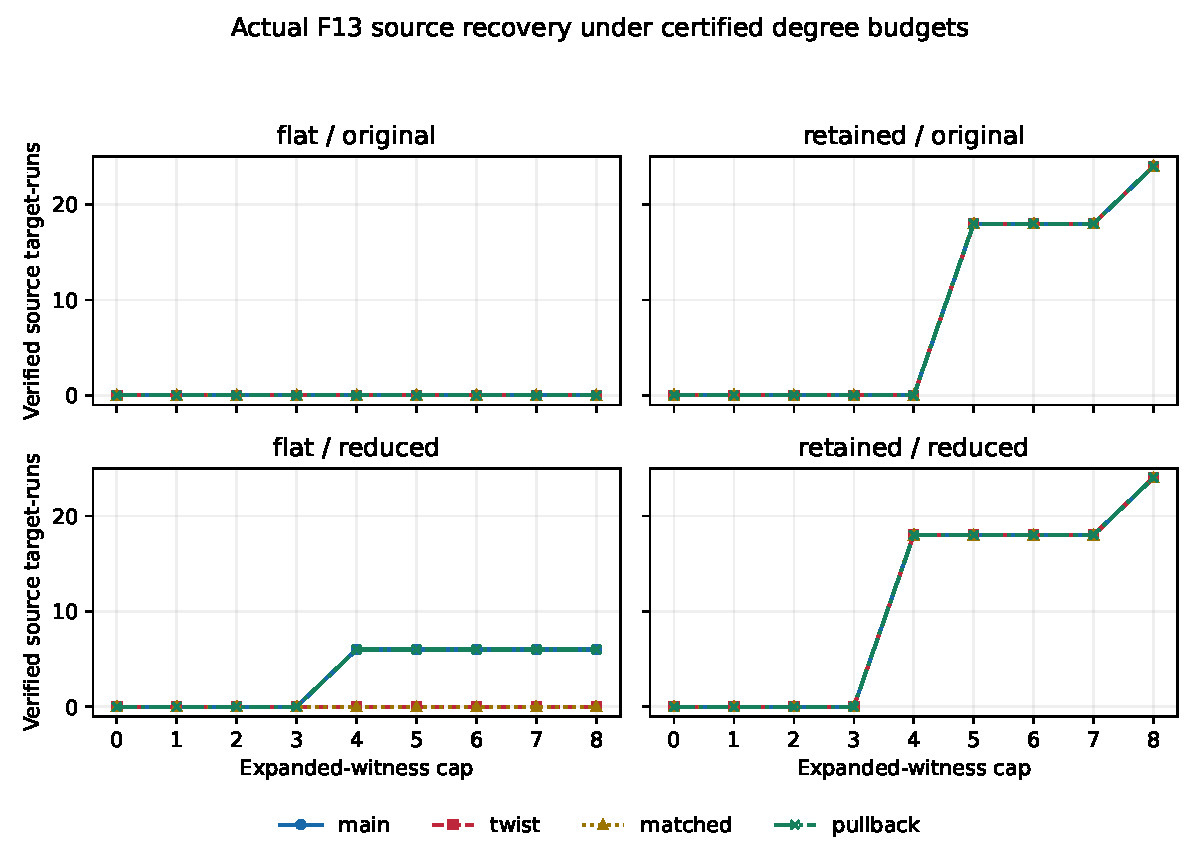
\includegraphics[width=\linewidth]{recovery.pdf}\end{center}
\textbf{Figure.} Native-recorded verified configuration-target runs per cap.
Each role contains four policies and six repeated separate targets (maximum24).
All values are exact; no sampling or timing uncertainty is inferred. Original
and reduced inputs, all losses and matched controls remain separate.

\textbf{Algebraic track.} The solver receives $S_3$ and both product-membership
polynomials. A flat Macaulay row has an explicit witness in these three inputs.
Acceptance requires a unit witness or bounded Gr\"obner certificate before root
extraction. A cap failure admits no roots; it does not prove the system empty.
Cartesian extraction and actual sign lifts happen only after certification.
Direct source enumeration is a separate generic-decomposition reference and
has no matrix-degree metric.

\textbf{Actual bound.} Both matrix row degree and expanded original-input
witness degree of verification must fit the rung. A shift above the bound is
denied before construction. Retained witnesses are local to one solve and
are reused only for an identical polynomial, with native ideal expansion
checked independently. All matrix work is still executed; a lower certificate
bound does not establish lower total cost.

\clearpage
{\Large Public setup, original scalar and remaining gates}
\begin{center}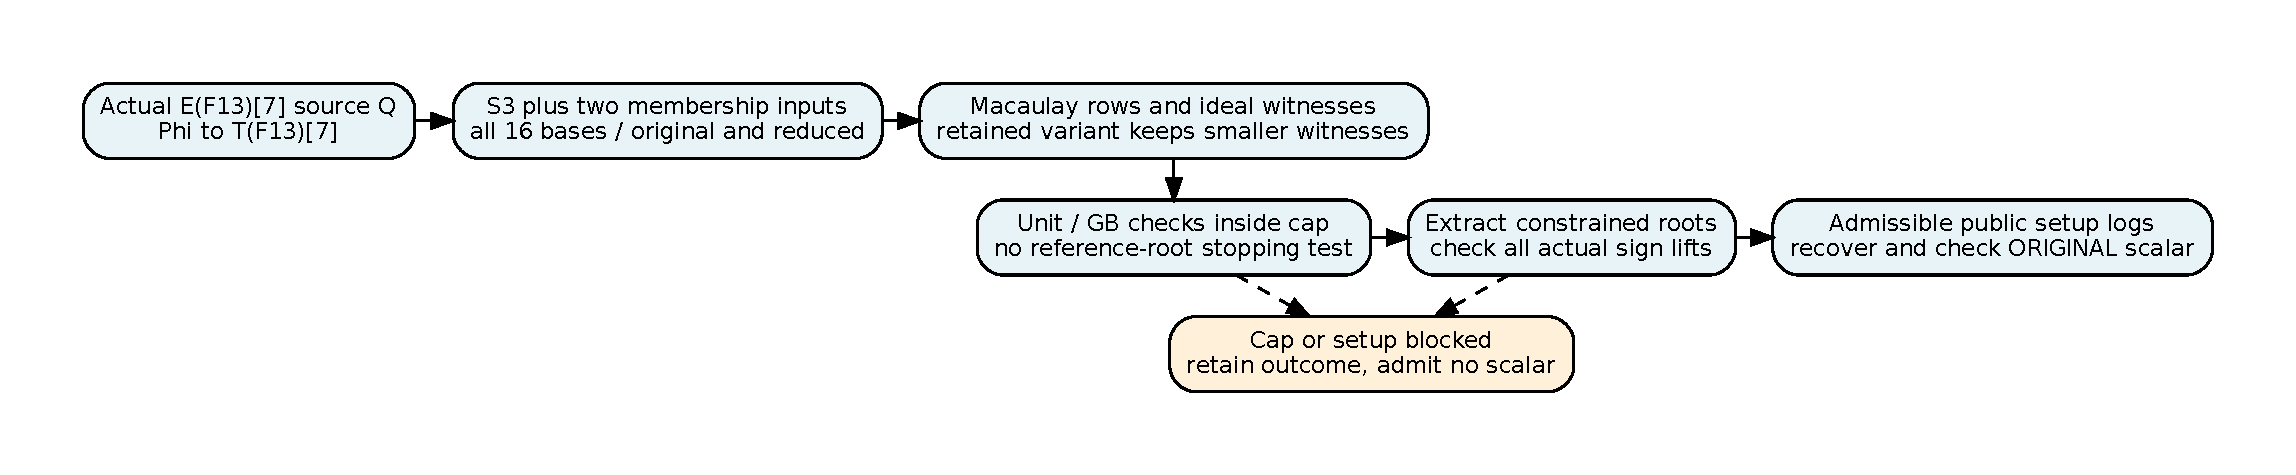
\includegraphics[width=\linewidth]{bridge.pdf}\end{center}
Only admitted public relations derive base logs; non-full-rank setups remain
blocked. Every accepted target relation uses actual unknown $Q$, all sign
lifts and failed shifts, then checks the scalar on original $E/P$.
The prior checked theorem, with explicit public $A_i=\ell_iU$, gives
\[
 \sum_i v_iA_i=\Phi(Q)+sU,\quad 7Q=0
 \quad\Longrightarrow\quad Q=\left(\sum_i v_i\ell_i-s\bmod7\right)P.
\]
That theorem and the old18polynomial identities are reused within their domains;
no new Lean/global audit or field-identity claim is made.

\textbf{Evidence.} Both full independent native replays pass; each set of nine
rehashed controls rejects101without a receipt and the same22backend tests pass
in each crate. All6251raw paths restore to exact hashes and repack. Duplicate
payloads restore from frozen canonical files; every altered payload remains.
Archive37124bytes and compressed manifest35984bytes meet policy. Four canonical
exports include both invalid attempts; none is hidden as a successful census.

\textbf{Limits and next lead.} The witness strategy is a finite certification
improvement; no strongest-source twist advantage or practical speedup. Setup,
field/group work, extraction, verification, allocation and external/rho pricing
are not a complete-cost result. Test a new transferable non-isomorphic fixture
or encoding against its entire source frontier after source/map verification.
No such new fixture search has run here.

\textbf{Completion hold.} Keep PR open, non-draft, auto-merge off. Missing study
registrations, naming, incomplete root library suite, required exact-headCI,
review, Conductor127/no lease, integration and broader geometry/probability/
regularity/full-work gates remain. No unrelated global gate or frozen evidence
changed. Existing local workers only;600second commands inside08:25--09:25UTC;
no paid provisioning or arbitrary result upload.

\small Sources and exact source/hash/flow/export links are in the adjacent
README and validation directory. Current protocols precede their affected
runs; the failed-audit repair and seen baseline are disclosed. Native witnesses
are finite polynomial records, not a universal verified solver theorem.
\end{document}
